\documentclass{exam}
%\documentclass[11pt,a4paper]{exam}
\usepackage{amsmath,amsthm,amsfonts,amssymb,dsfont}
\usepackage{ifthen}
\usepackage[legalpaper, total={177.8mm, 290mm}]{geometry}
\usepackage{enumerate}% http://ctan.org/pkg/enumerate
\usepackage{multicol}
\usepackage{graphicx}



% Accumulate the answers. Unmodified from Phil Hirschorn's answer
% https://tex.stackexchange.com/questions/15350/showing-solutions-of-the-questions-separately/15353
\newbox\allanswers
\setbox\allanswers=\vbox{}

\newenvironment{answer}
{%
    \global\setbox\allanswers=\vbox\bgroup
    \unvbox\allanswers
}%
{%
    \bigbreak
    \egroup
}

\newcommand{\showallanswers}{\par\unvbox\allanswers}
% End Phil's answer


% Is there a better way?
\newcommand*{\getanswer}[5]{%
    \ifthenelse{\equal{#5}{a}}
    {\begin{answer}\thequestion. (a)~#1\end{answer}}
    {\ifthenelse{\equal{#5}{b}}
        {\begin{answer}\thequestion. (b)~#2\end{answer}}
        {\ifthenelse{\equal{#5}{c}}
            {\begin{answer}\thequestion. (c)~#3\end{answer}}
            {\ifthenelse{\equal{#5}{d}}
                {\begin{answer}\thequestion. (d)~#4\end{answer}}
                {\begin{answer}\textbf{\thequestion. (#5)~Invalid answer choice.}\end{answer}}}}}
}

\setlength\parindent{0pt}
%usage \choice{ }{ }{ }{ }
%(A)(B)(C)(D)
\newcommand{\fourch}[5]{
    \par
    \begin{tabular}{*{4}{@{}p{0.23\textwidth}}}
        (a)~#1 & (b)~#2 & (c)~#3 & (d)~#4
    \end{tabular}
    \getanswer{#1}{#2}{#3}{#4}{#5}
}

%(A)(B)
%(C)(D)
\newcommand{\twoch}[5]{
    \par
    \begin{tabular}{*{2}{@{}p{0.46\textwidth}}}
        (a)~#1 & (b)~#2
    \end{tabular}
    \par
    \begin{tabular}{*{2}{@{}p{0.46\textwidth}}}
        (c)~#3 & (d)~#4
    \end{tabular}
    \getanswer{#1}{#2}{#3}{#4}{#5}
}

%(A)
%(B)
%(C)
%(D)
\newcommand{\onech}[5]{
    \par
    (a)~#1 \par (b)~#2 \par (c)~#3 \par (d)~#4
    \getanswer{#1}{#2}{#3}{#4}{#5}
}

\newlength\widthcha
\newlength\widthchb
\newlength\widthchc
\newlength\widthchd
\newlength\widthch
\newlength\tabmaxwidth

\setlength\tabmaxwidth{0.96\textwidth}
\newlength\fourthtabwidth
\setlength\fourthtabwidth{0.25\textwidth}
\newlength\halftabwidth
\setlength\halftabwidth{0.5\textwidth}

\newcommand{\choice}[5]{%
\settowidth\widthcha{AM.#1}\setlength{\widthch}{\widthcha}%
\settowidth\widthchb{BM.#2}%
\ifdim\widthch<\widthchb\relax\setlength{\widthch}{\widthchb}\fi%
    \settowidth\widthchb{CM.#3}%
\ifdim\widthch<\widthchb\relax\setlength{\widthch}{\widthchb}\fi%
    \settowidth\widthchb{DM.#4}%
\ifdim\widthch<\widthchb\relax\setlength{\widthch}{\widthchb}\fi%

% These if statements were bypassing the \onech option.
% \ifdim\widthch<\fourthtabwidth
%     \fourch{#1}{#2}{#3}{#4}{#5}
% \else\ifdim\widthch<\halftabwidth
% \ifdim\widthch>\fourthtabwidth
%     \twoch{#1}{#2}{#3}{#4}{#5}
% \else
%      \onech{#1}{#2}{#3}{#4}{#5}
%  \fi\fi\fi}

% Allows for the \onech option.
\ifdim\widthch>\halftabwidth
    \onech{#1}{#2}{#3}{#4}{#5}
\else\ifdim\widthch<\halftabwidth
\ifdim\widthch>\fourthtabwidth
    \twoch{#1}{#2}{#3}{#4}{#5}
\else
    \fourch{#1}{#2}{#3}{#4}{#5}
\fi\fi\fi}


\begin{document}

\begin{table}[h]
\centering
\begin{tabular}{lllll}
\textbf{\large SYLHET CADET COLLEGE} &  &  &  &  \\ \cline{4-5} 
PRE-TEST EXAMINATION - 2023 &  & \multicolumn{1}{l|}{} & \multicolumn{1}{l|}{Set} & \multicolumn{1}{l|}{:A} \\ \cline{4-5} 
CLASS: XII &  &  &  &  \\ \cline{3-5} 
MULTIPLE CHOICE QUESTIONS & \multicolumn{1}{l|}{\textbf{Subject Code:}} & \multicolumn{1}{l|}{1} & \multicolumn{1}{l|}{2} & \multicolumn{1}{l|}{9} \\ \cline{3-5} 
STATISTICS FIRST PAPER &  &  &  &  \\
TIME – 25 minutes &  &  &  &  \\
FULL MARKS – 25 &  &  &  & 
\end{tabular}
\end{table}
%  \normalfont\normalsize
 % 11.45a.m.~--~1.45p.m.
\hrule

\begin{center}
[N.B. – Answer all the questions. Each question carries ONE mark. Block fully, with a black ball- point pen, the circle of the letter that stands for the correct/best answer in the “Answer sheet” for the Multiple Choice Questions Examination.]\\

  
  \textbf{Candidates are asked not to leave any mark or spot on the question paper.}
\end{center}
\begin{questions}


\question \textbf{Which cannot be performed using Univariate data?}
\choice{Central tendency}{Dispersion}{Skewness}{Regression}{d}

\question \textbf{Cities ranked according to habitability level show -- measurement scale}
\choice{Nominal}{Ratio}{Interval}{Ordinal}{d}

\question \textbf{Which of the following is correct?}
\choice{$\displaystyle \sum_{i=1}^{20} cx_i = nc \sum_{i=1}^{20} x_i$}{$\displaystyle \sum_{i=1}^{20} cx_i = nc \sum_{i=1}^{20} x_i$}{$\displaystyle \sum_{i=1}^{20} cx_i = c \sum_{i=1}^{20} x_i$}{$\displaystyle \sum_{i=1}^{20} cx_i = c^2 \sum_{i=1}^{20} x_i$}{b}

\question \textbf{Which is not an example of shift of scale?}
\choice{$y_i = \frac{x_i}{a}$}{$y_i = cx_i$}{$y_i = x_i-2$}{$y_i = \frac{cx_i}{d}$}{a}

\question \textbf{Which measure of central tendency is suitable for qualitative variable?}
\choice{Arithmetic Mean}{Harmonic Mean}{Quadratic Mean}{Mode}{d}

\question \textbf{From the following table, $\displaystyle \sum_{i=1}^4 x_iy_i=?$}

\begin{table}[h]
\centering
\begin{tabular}{c|c|l|c|l}
X & 1  & 5  & 3 & 2  \\ \hline
Y & 20 & 12 & 3 & 14
\end{tabular}
\end{table}

\choice{14}{201}{99}{117}{d}


\question \textbf{Arithmetic Mean is --}

i. Rigidly defined \\
ii. Unaffected by sample fluctuation \\
iii. Suitable for algebraic analysis

\textbf{Which one is correct?}

\choice{i and ii}{i and iii}{ii and iii}{i, ii and iii}{b}

\textbf{Answer the next two (2) questions based on the following information}

\begin{table}[h]
\centering
\begin{tabular}{c|c|c|c|c|c|c}
Class                                                           & $\le 20$ & 20-25 & 25-50 & 50-60 & 69-70 & $\ge 70$ \\ \hline
Frequency                                                       & 5        & 10    & 10    & 7     & 5     & 3        \\ \hline
\begin{tabular}[c]{@{}c@{}}Cumulative \\ Frequency\end{tabular} & 5        & 15    & 25    & 32    & 37    & 40      
\end{tabular}
\end{table}

\question \textbf{How many values are between 20 and 70?}
\choice{20}{32}{35}{37}{b}

\question \textbf{Which one is the median class?}
\choice{20-25}{25-50}{50-60}{60-70}{b}

\question \textbf{In presence of negative values, which measure is not usable?}
\choice{Arithmetic Mean}{Geometric Mean}{Quadratic Mean}{Harmonic Mean}{b}

\question \textbf{For grouped data, which formula is correct for Arithmetic Mean?}
\choice{$\displaystyle \bar x = \frac{\sum f_ix_i}{\sum f_i}$}{$\displaystyle \bar x = \frac{\sum x_i}{N}$}{$\displaystyle \bar x = \frac{\sum f_ix_i}{n}$}{$ \displaystyle\bar x = \frac{\sum f_i}{N}$}{a}

\question \textbf{Arithmetic mean of the series 2, 12, 22, $\cdots$, 92 is--}
\choice{45}{46}{47}{55}{c}

\question \textbf{Median can be determined from the--}
\choice{Histogram}{Frequency curve}{Ogive}{Pie Chart}{c}

\question \textbf{Which statement is correct}
\choice{Quartiles are well defined}{Outliers affect Median}{Median is always present in data}{Quadratic mean is widely used}{a}

\question \textbf{The formula of coefficient of variance (CV) is --}
\choice{$\frac{\mu_2}{n}\times 100$}{$\frac{\mu_2}{\mu_1}\times 100$}{$\frac{\mu_2}{\bar x}\times 100$}{$\frac{\mu_3}{\sigma}\times 100$}{c}

\question \textbf{Which measure is unit-free?}
\choice{Range}{Mean deviation}{Standard deviation}{Coefficient of variation}{d}

\question \textbf{Which is not a type of Moments}
\choice{Central Moments}{Raw Moments}{Corrected Moments}{Rectified Moments}{d}

\question \textbf{The second moment around w is --}
\choice{$\frac{\sum (x_i-\bar x)^n}{w}$}{$\frac{\sum (x_i-\bar x)^2}{w}$}{$\frac{\sum (x_i-w)^2}{n}$}{$\frac{\sum (x_i-w)^n}{2}$}{a}

\question \textbf{The following graph is an example of --}

\begin{center}
   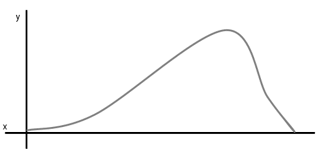
\includegraphics[width=0.2\textwidth]{../img/neg_skew.png}
\end{center}

\choice{Positive Skew}{Negative Skew}{No Skew}{Not detectable}{a}

\question \textbf{Which formula is correct for determining skewness?}
\choice{$\gamma_1 = \sqrt{\frac{\mu_3^2}{\mu_2^3}}$}{$\gamma_1=\sqrt{\beta_1^2}$}{$\gamma_1 = \sqrt{\frac{\mu_3}{\mu_2^3}}$}{$\frac{\mu_2}{\sqrt{\mu_3^2}}$}{a}

\question \textbf{A linear trend goes along a -- }
\choice{a curved line}{a wave}{straight line}{circle}{a}

\textbf{Answer the next THREE questions based on the following information}

\begin{table}[h]
\begin{tabular}{c|cccccccc}
Year & 2016 & 2017 & 2018 & 2019 & 2020 & 2021 & 2022 & 2023 \\ \hline
USD Exchange Rate & 78.35 & 79.49 & 82.87 & 83.26 & 84.60 & 84.37 & 85.80 & 106.70
\end{tabular}
\caption{\label{usdrate}Source--Investing.com}
% https://www.investing.com/currencies/usd-bdt-historical-data
\end{table}

\question \textbf{What is the second value of semi-average method?}
\choice{85.40}{90.37}{91.73}{89.78}{b}

\question \textbf{What kind of a trend do the data have?}
\choice{Upward}{Downward}{Both upward \& downward}{No trend}{a}

\question \textbf{Which component of time series is visible in the later part of the data?}
\choice{Seasonal Variation}{General Trend}{Irregular Variation}{Cyclic Variation}{c}

\question \textbf{Limitations of published statistics in Bangladesh are --}

i. Wrong data collection method \\
ii. Insufficient data \\
iii. Lack of proper training

\textbf{Which one is correct?}

\choice{i and ii}{i and iii}{ii and iii}{i, ii and iii}{d}

%\question \textbf{To complete the song, the last answer should be
%\choice{a}{b}{c}{d}{e} % Invalid answer choice

\end{questions}

\pagebreak
%\newpage  %Uncomment to put on new age
\bigskip

\begin{multicols}{3}
[
Answer Key
]
\showallanswers % Phil Hirschorn
\end{multicols}


\end{document}